\documentclass{beamer}
\usepackage[utf8]{inputenc}
%\usepackage[russian]{babel}
\usepackage{amsmath,mathrsfs}
\usepackage{graphicx, epsfig}
\usetheme{Warsaw}%{Singapore}%{Warsaw}%{Warsaw}%{Darmstadt}
\usecolortheme{sidebartab}
\usepackage{graphicx}
\definecolor{beamer@blendedblue}{RGB}{15,120,80}
%----------------------------------------------------------------------------------------------------------
\title[\hbox to 56mm{Feature generation  \hfill\insertframenumber\,/\,\inserttotalframenumber}]
{TOUCH: In-Memory Spatial Join by Hierarchical Data-Oriented Partitioning}
\author[A.\,Logins]{\large \\A.\, Logins}
\institute{\large
Moscow Institute of Physics and Technology\par
Skolkovo Institute of Science and Technology}

\date{\footnotesize{\emph{Course:} Machine Learning and Data Analysis\par (Strijov's practice)/Group 174, 2014 Fall}}
%----------------------------------------------------------------------------------------------------------
\begin{document}
%----------------------------------------------------------------------------------------------------------
\begin{frame}
%\thispagestyle{empty}
\titlepage
\end{frame}
%-----------------------------------------------------------------------------------------------------
\begin{frame}{Goal of research}
\begin{block}{Motivation}
Develop In-Memory Spatial Join algorithm with Iterative Hierarchical Data-Oriented Partitioning with balanced workload
\end{block}
\end{frame}
%----------------------------------------------------------------------------------------------------------
\begin{frame}{Problem statement}
Given the parameter $\epsilon$ two datasets of spatial objects $A$ and $B$ find all $a\in A$ and $b \in B$ such that minimum distance between them is less than $\epsilon$.
\end{frame}
%----------------------------------------------------------------------------------------------------------
\begin{frame}{Solution}
\begin{itemize}
\item Build Hilbert curve through all MBRs of spatial objects (create index)
\item Build R-tree through indexed MBRs, maintaining MBRs of two types (according to types of objects) for each node
\item For each leaf node take objects and assign to the nodes of the tree, dynamically updating MBRs and deleting them from the leaf nodes
\item  For each node join assigned objects with object assigned below
\end{itemize}
\end{frame}
%----------------------------------------------------------------------------------------------------------
\begin{frame}{Computational experiment}
\begin{figure}[p]
    \centering
    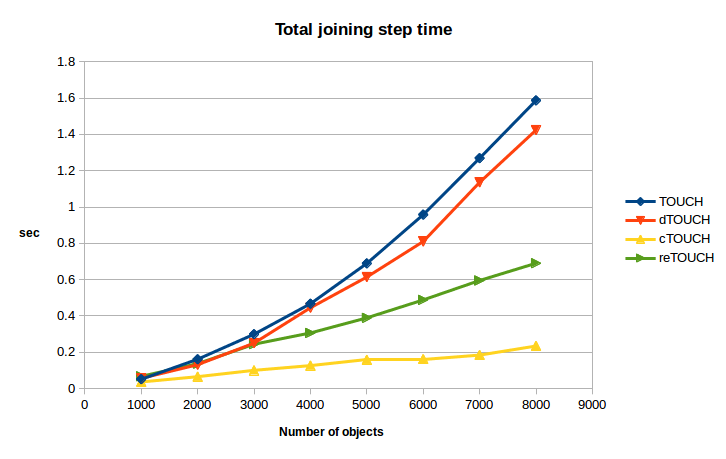
\includegraphics[width=0.8\textwidth]{Images/joinTime.png}
\end{figure}
\end{frame}
\begin{frame}{Computational experiment}
\begin{figure}[p]
    \centering
    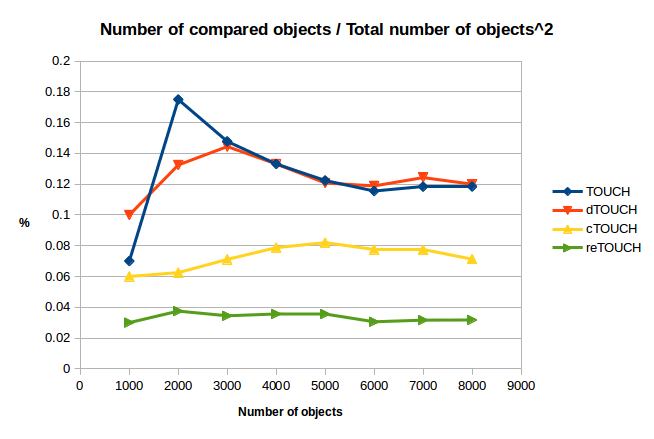
\includegraphics[width=0.8\textwidth]{Images/compObj.png}
\end{figure}
\end{frame}
%----------------------------------------------------------------------------------------------------------
\begin{frame}{Conclusion}
Two of three new approaches give considerable improvement in performance and number of comparisons.
\end{frame}
%----------------------------------------------------------------------------------------------------------
\end{document} 